%  University of Houston PhD proposal
%
% on  PC
%\documentclass[12pt]{report}
% \usepackage{uhthesis}
% \usepackage[pctex32]{graphics}
% \usepackage[pctex32]{color}
%\usepackage{psfig}
\documentclass[12pt]{report}
\usepackage{uhthesis3}
\usepackage{epsfig}
\usepackage{epsf}
\usepackage{listings}
\usepackage{array}
\usepackage{subcaption}
\usepackage[font=footnotesize]{subfig}
\usepackage{float}
%\usepackage[]{algorithm2e}
\input{definitions.tex}
%\input{algorithms}
%
%
%
% on UNIX LATEX and Windows PCTEX32
%\documentstyle[12pt,uhthesis1,psfig]{report}
%\usepackage{epsfig}
%\input{algorithms}
%\input{psfig}
%\input{dnmmath}
%\input{ion-math}
\newcolumntype{L}[1]{>{\raggedright\let\newline\\\arraybackslash\hspace{0pt}}m{#1}}
\setcounter{secnumdepth}{4}
\begin{document}

\title{\bf \large Implementation and evaluation of Addtional Parallel Features in Coarray Fortran}
\author{Shiyao Ge}
\submitdate{May 2016} \degree{Masters}{Proposal}
\adviser{Barbara Chapman, Chairman\\
Dept. of Natural Sciences \& Mathematics }

\firstreader{Edgar Gabriel \\
Dept. of Natural Sciences \& Mathematics }

\secondreader{Mikhail Sekachev\\
TOTAL E\&P Research and Technology USA, LLC}
 \threereadersfalse
 \fourreadersfalse
  \fivereadersfalse
\copyrightfalse \makecoverpages
\begin{acknowledgements}
%\input{acknowledgements.tex}
\end{acknowledgements}

\begin{abstract}
\input {abstract.tex}
\end{abstract}
\setlength{\parskip}{.1 in}

\makecontentspages

%uncomment the following for single space drafts
%\singlespace

% \pagenumbering{romans}{1}
% \beforepreface

%\pagestyle(empty}


%%%%%%%%%%%%%%%%%%%%%%%%%%%%%%%%%%%%%%%%%%%%%%%%%%%%%%%%%%%%%%%%%%%%


% \input{chapter0Nomenclature.tex}
% \setcounter{page}{0}

\chapterpages

%turn figures on and off
\newif \ifFIGS

%\FIGStrue

\FIGSfalse
%TODO: delete plain page before abstract

% to fix the page number
%\input{Sample_chapter.tex}
%\input{table.tex}
\chapter{Introduction}\label{chap:Intro}
\begin{itemize}
\item The work is important.
\item What is the current situation for HPC and Coarray Fortran
\item My contribution in this work
\item Following organizations
\end{itemize}
\chapter{Background}\label{chap:Background}
\section{FORTRAN in HPC}
\section{Team based parallel construct}
\section{Previous work}
\chapter{Infrastructure}\label{chap:Methods}
\section{OpenUH compiler}
OpenUH\cite{liao2007openuh}\cite{chapman2013experiences} is a branch of the open-source Open64 compiler suite which researchers in the HPCTools group at the University of Houston have developed and used to support a range of research activities in the area of programming model research. In figure~\ref{fig:openuhcompiler} shows the overall compiler infrastructure for OpenUH. Its modern and complete framework for inter- and intra-procedural state-of-art analyses and optimization is the most prominent part of Open64/OpenUH. OpenUH uses a tree-based IR called WHIRL. It comprises 5 levels, from Very High(VH) to Very Low(VL), to enable a broad range of optimizations. This design allows the compiler to perform various optimizations with proper form of IRs on different levels. 
\begin{figure}
\centering
\label{fig:openuhcompiler}
\includegraphics[scale=0.6]{figures/openuharchitecture}
\caption{OpenUH compiler infrastructure}
\end{figure}
The major functional parts of the compiler that we may concern are the C/C++ frontend and Fortran frontend, the interprocedural analyzer/optimizer(IPA/IPO) and the middle-end/back-end, which is further subdivided into the loop nest optimizer(LNO), glboal optimizer(WOPT), and code generators(CG) for 32-bit and 64-bit x86 platforms. Addtional features provided by this compiler infrastructure include the ability to emit source from an optimized intermediate representation, as well as to selectively instrument the lowered intermediate code for low-overhead performance profiling. 

The HPCTools group has undertaken a broad range of infrastructure development in OpenUH to support important topics such as language research, static analysis of parallel programs, performance analysis, task scheduling, and dynamic optimization, etc\cite{}.

OpenUH provided a solid base infrastructure for exploring implementation strategies for Coarray Fortran. The Fortran 95 frontend, which is contributed by Cray, was already capable to recognize coarrays and parsing the cosubscript syntactic extension. We took it as the start point for our implementation. The multi-level WHIRL IR, used throughout the middle-end and back-end of the compiler, provides rich support for a wide range of program abstractions. At its highest level of abstraction, VH-WHIRL, it is capable of representing Fortran array sections. This allowed us to design our back-end translator to directly map array section remote memory access into bulk communication function calls. The comprehensive optimization infrastructure available in OpenUH also provides a means for us to generate highly optimized coarray programs. OpenUH also includes its own Fortran runtime libraries, providing support for the myriad intrinsic routines defined in Fortran, memory allocation, I/O, and program termination. We chose to implement our CAF runtime outside these othter Fortran runtime libraries and reduce as much as possible its dependence on them. This would allow us to very easily port our CAF runtime to be used with different compiler.

\section{Coarray Fortran}\label{sec:coarrays}
In chapter~\ref{chap:Background} we have gone through the history of Fortran and currently active Coarray Fortran project. In this section, we will have a closer look to the parallel features that are defined and will be included in the latest Fortran language specification. 

Coarray Fortran(CAF) is a subset of the Fortran 2008 standard which adds parallel processing capabilities to the base language by adopting a SPMD model for work decomposition and \emph{coarrays} for data decomposition. In following subsections, we will go through the enssential parts of this parallel language and see some syntax examples when necessary. 

\subsection{Execution Unit}
In Coarray Fortran program, the execution unit is called \emph{image}. A Coarray Fortran program is consist a set of \emph{images} which are lanching at the beginning of program and running in parallel. The number of \emph{images} can be specified ahead of programming running but it is fixed during the execution of the program. One can set this number via compiler option, by an environement variable, or specified by options passed to a program job launcher. Each image is identified by an unique image index which start from 1 to the number of images. Two intrinsic functions \texttt{this\_image} and \texttt{num\_images} are provided for user to query about the \emph{image} identification and total number of images running during the program. Pratically, each running image is running on a separate processor but it is not necessary, and it performs computations on the data residing in its local memory. Part of images' memory are shared between images, which means other images may access to other images' memory space with a one-sided communication manner.  

\subsection{Coarrays}
These logically shared memory object are decleared and represented in CAF program as \emph{Coarrays}. Coarrays are declared with the \texttt{codimension} attribute specifier. Codimensions are analogous to array dimensions, in that they may be used to describe a multi-dimensional rectangular shape associated with a data entity. Codimensions describes the rectangular \emph{coshape} of the set of images which each contain the coarray variable in its memory. 

Coarrays may be tranfered as dummy arguments into a procedure, so long as the associated actual argument is also a coarray. Otherwise, a coarray may be decleard with either the \texttt{save} or \texttt{allocatable} attribute, for static coarrays and dynamic allocatable coarrays respectively. For non-allocatable coarrays, the \texttt{codimension} specifier should indicate the size of all codimensions except the last one for which the upper-bound must be specified as an asterisk, as shown in figure~\ref{fig:coarraydemo}. Allocatable coarrays have a \emph{deferred} coshape; the dimension bounds should specified in the \texttt{allocate} statement with the last codimension specified with an asterisk. 

Codimensions associated with a coarray provide a means to uniquely refer to a coarray located on another image, which we called \emph{image selection}. When a coarray variable is referenced with \emph{cosubscript}, similar as subscript to array selection syntax but surrounded within square brackets, the compiler will identify it as a remote memory access to the coarray at the image identified by the cosubscripts. The intrinsic functionn \texttt{image\_index} will return the image index of the image containing a specified coarray variable with a specified set of cosubscripts. Unlike the array reference, cosubscripts must uniquely refer to a single image. It cannot use subscript triplets and vector subscripts to refer more than one images at once. In Fortran, a data oject is remote accessible if it is (1) a coarray, (2) a pointer or allocatable component of a coarray, or (3) an object with the \texttt{target} attribute that is pointer associated with a pointer component of a corrary. 

\subsection{Image Control Statement}
%TODO:EDIT this part
\subsection{Teams and collectives}
As we discussed in section~\ref{sec:caf2.0}, the features in Fortran 2008 standard only provides a simple set of syntax for expressing communication and basic coordination mechanism among excuting images. The researcher in Rice University have proposed a set of new constructs and syntax to extend the CAF. Recently, the Fortran Standard committee is working on the addtional parallel features, which are described in the technical specification document\cite{caf-spec}. In this draft, they propose some language features to deal with the shortage that we have discussed in section~\ref{sec:caf2.0}. Among these features, the \emph{team} and \emph{collectives} are going to be the main topic in this thesis. We will talk about them in detail in chapter~{chap:Algorithms}.

%Researchers in Rice University have proposed their notation for subset of processes, named as \emph{team}. In the specification, the Fortran work group have proposed a similar construct, also named as \emph{team}. In the beginning of CAF program, all images are launched and included into the \emph{initial team}. During the program, all images may create a new team with \texttt{form team} statement. This statement will split current team into several \emph{sibling team}, according to the \emph{team\_id} they have specified to the statement. All the images in the current team are uniquely assigned to one of those teams. In CAF 2.0, the routine provides similar functionality is \texttt{team\_split}. Each image have a private \emph{team variable} to store the necessary information.

%Another important feature introduced into language is the collective functions. 

\subsection{Termination}
A Coarray Fortran program may terminate in one of two modes - \emph{normal terminination} or \emph{error termination}. When an image reaches to the end of a program or executes the stop statement, it will terminate properly in three steps: initiation, synchronization and completion. One image cannot terminated until all images reach the second step of normal completion. Error termination occurs when an image meets an error condition. This could occur when it encounters an error state as defined by the standard, when the program executed an \texttt{error stop} statement, or maybe it is notified that some other image is in error termination. When any image initiates error termination, the runtime should attempt to signal all images as soon as possible to shut them down and return an error status code.
\subsection{Other features}
To be noticeed that there are some other useful features or syntax on the specfication and we have supported in our compiler and runtime. I will name some of them here but I cannot go further detail about them since they are less relevent to my topic in this thesis. 

We have supported Atomic object and operations upon them. 
%TODO: EDIT: ATOMIC, EVENT
\section{GASNet}
In our CAF runtime, we chose two outstanding libraries as our communication layer, GASNet and ARMCI. In this thesis, I will only focus on the first one, GASNet, since most of my work is done and verified on top of it. GASNet\cite{bonachea2002gasnet}\cite{bonachea2002gasnetspec}, for the abbreviation of Global Address Space Networking library, is a language indenpendent runtime library developed and maintained by a research group at the University of California Berkeley and Lawrence Livermore National Laboratory. GASNet was designed to serve the UPC and Titanium, which are two famous PGAS languages with base language in C and Java. Soon it has been widely used to support a variety of PGAS implementations inluding the Co-Array Fortran and CAF 2.0 from Rice University. We also found it in Cray's UPC and CAF compiler for the CrayXT series, the Cray Chapel compiler and OpenSHMEM reference implementation, which is developed and maintained by Univeristy of Houston. 

GASNet has an API specification which defines interface for compilers or runtime system to use, which we will briefly review in this section. GASNet was designed with portability and performance in mind, and it includes implementations for many popular network APIs covering the common cluster interconnects, as well as specialized interconnects from IBM and Cray. 

A running program which uses GASNets, called the client program, consists of a set of operating system processes, or \emph{nodes}. These nodes may furthermore be grouped into supernodes, which means they are controlled by the same operating system instance. Each node may attach a \emph{segment} to its address space, which is a range of virtual addresses that are remotely access across GASNet nodes. Furthermore, the client program may execute in one of three threading modes 
\begin{itemize}
\item GASNET\_SEQ allows only one single thread on a node the make any GASNet calls
\item GASNET\_PARSYNC allos only one thread to make GASNet calls at a time
\item GASNET\_PAR provides full multi-threaded support
\end{itemize}

The GASNet API consists of a core API and an extended API. The core API provides all the facilities necessary to manage parallelism in the application, including runtime initialization and finalization, querying the environment variables in GASNet, and mutexes for multi-threaded client programs. In this thesis, the most significant part of the core API is the \emph{active message}(AM) support. This provides means to invoke registered AM handlers on a remote GASNet node. The handlers are resricted to using only a subset of the core API, and in particular they may not use the extended API for communicating with other GASNet nodes. The core API also provides support for named or unnamed split-phase barriers. 

The extended API provides support for remote memory access(RMA) operations. This includes blocking \emph{get} and \emph{put} operations, implicit-handle non-blocking \emph{get} and \emph{put}, and explicit-handle non-blocking Get and Put, and synchronization routines for waiting on completion of explicit-handle and implicit handle RMA operations. While the specificaion presently allows only contiguous remote data transfers, we can also find support for non-contiguous remote data transfer in Berkeley's implementation. 



\chapter{Implementation}\label{chap:Algorithms}
\section{Baseline Team Implemenation} 
In this section, I will describe the addtional features described in the Techinical Specification draft and the implementation we made in the OpenUH compiler. 
Previously, we implemented support for Fortran coarrays in OpenUH in accordance with the Fortran 2008
specification~\cite{EachempatiCoarray2013}~\cite{EachempatiCAF2010}.  The OpenUH Coarray Fortran implementation is depicted in Figure~\ref{fig:teams-openuh}.  

\begin{figure}[!h]
\centering
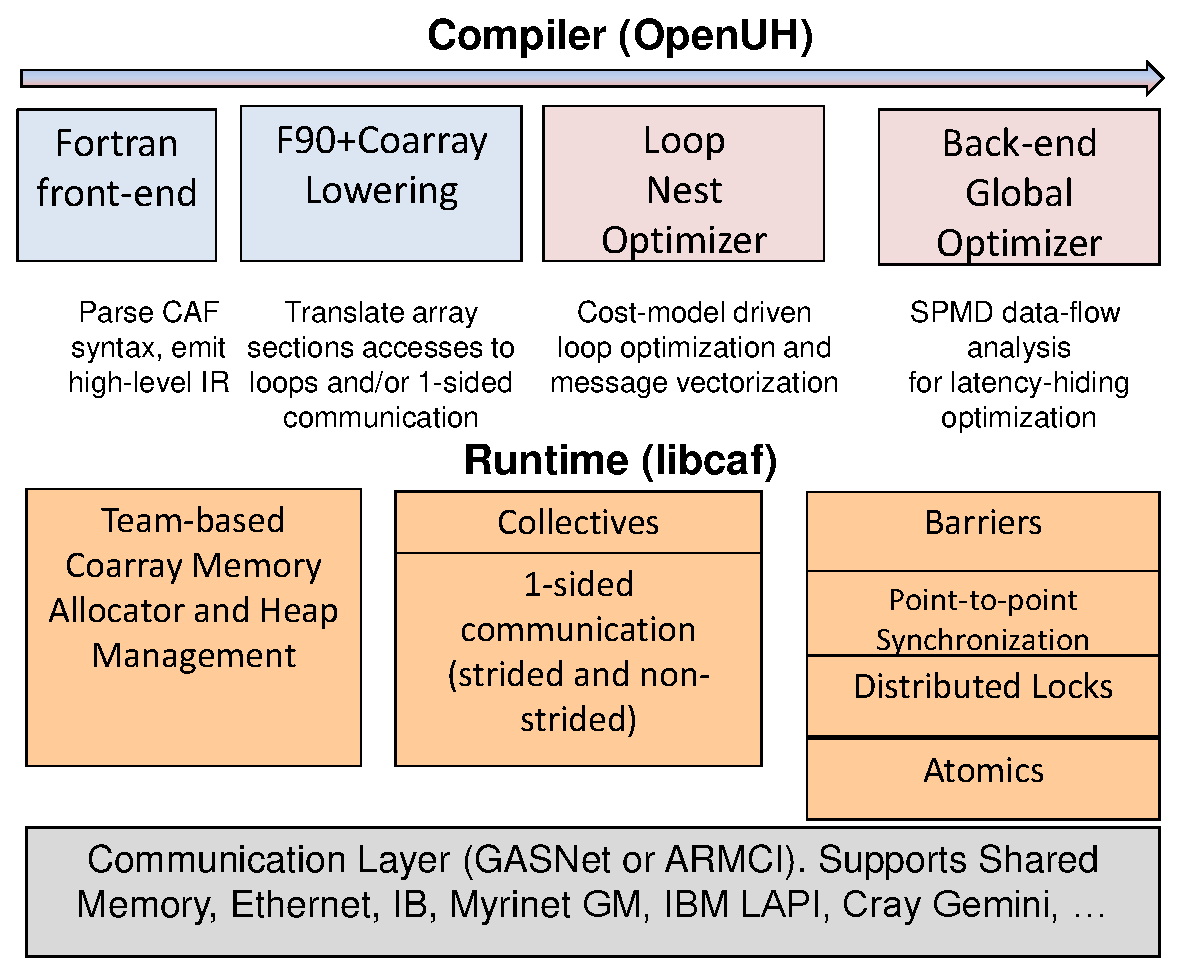
\includegraphics[width=5in, height=4in]{figures/uh-coarrays-implementation-stack.eps}
% where an .eps filename suffix will be assumed under latex, 
% and a .pdf suffix will be assumed for pdflatex; or what has been declared
% via \DeclareGraphicsExtensions.
\caption{OpenUH Coarray Fortran team implementation}
\label{fig:teams-openuh}
\end{figure}

%\subsection{Runtime Design and Implementation for Teams} 

We added support into the Fortran front-end of OpenUH for parsing the
\texttt{form team},  \texttt{change team}, \texttt{end team} and \texttt{sync
team} constructs. We added the new type \texttt{team\_type} to the type system
of OpenUH and support for \texttt{get\_team} and \texttt{team\_number} intrinsics.
We also extended  the CAF intrinsics \texttt{this\_image},
\texttt{num\_images}, and \texttt{image\_index} for teams.
During the back-end compilation process in OpenUH, team-related constructs are
lowered to subroutine calls which constitute the \textit{libcaf} runtime
library interface. In the runtime, we added a \texttt{team\_type} data structure
for storing image-specific identification information, such as the mapping
from a new index to the process identifier in the lower communication layer.
The runtime also provides support for the team-related intrinsics
\texttt{get\_team} and \texttt{team\_number}.


Before team support was added into our implementation, coarray allocation was
globally symmetric across all images, with each coarray allocated at the same
offset within a managed symmetric heap.

With teams, however, this global symmetry is no longer necessary. According to the
draft of the technical specification, symmetric data objects have the
following features, which simplify the memory management for teams. First,
whenever two images are in the same team, they have the same memory
layout. Second, an image can only change to the initial team or teams formed
within  the current team. Third, when exiting a given team, all coarrays
allocated within this team should be deallocated automatically. And fourth, if
an image needs to refer to a coarray of another image located in a sibling
team, the coarray should be allocated in their common ancestor team.

Team variables are opaque, first-class objects which may be used to query
information for a specified team or change to a specified team. In our
implementation, a team variable refers to an associated team data structure,
depicted in Table~\ref{team-ds}. During the formation of a team, the values
for the fields of this data structure are computed and populated, including
(1) the list of images that are on the same node, (2) the number of images
within the same node, and (3) fields used to facilitate execution of
collective operations.  This information is used many times in the runtime by
different parallel algorithms (for example, collectives and barriers as
described in Section~\ref{sec:collectives}).
\begin{table}[!h]
%\begin{minipage}{1\columnwidth}%{\columnwidth}
%\centering

\caption{Team data structure}
\label{team-ds}
%\centering
%\hspace*{0.5in}

\begin{tabular}{|c|L{4.2in}|}
\hline
\textbf{Field} & \textbf{Description}  \\ 
\hline

 team\_num          & a team number or id, assigned during \texttt{form team} statement\\ \hline
 this\_image        & image index for current image in team \\ \hline
 num\_images        & number of images in team \\ \hline
intranode\_set      & ordered list of image indices in same compute node\\\hline
leader\_set         & ordered list of image indices of node leaders in team\\\hline
 leaders\_count     & number of node leaders in team\\\hline
 image\_index\_map  & maps image index to image index in inital team\\ \hline 
 sibling\_maps      & image index mapping for each sibling team created by same \texttt{form team} statement \\\hline
 bar\_parity                  & parity variable for dissemination barrier\\\hline 
bar\_sense                   & sense variable for dissemination barrier\\\hline
intranode\_bar\_flags        & direct shared pointers to intra-node barrier partners' flags\\\hline
bar\_rounds\_info            & partner information for inter-node in dissemination barrier rounds \\\hline
coll\_sync\_flags            & bcast, reduce, and allreduce sync flag\\     \hline
allreduce\_bufid             & selects between two allreduce buffers\\\hline
 reduce\_bufid                & selects between two reduce buffers\\\hline
 bcast\_bufid                 & selects between two bcast buffers \\\hline
 allocations     & a list of symmetric memory slots allocated for this team\\\hline 
 parent  		 & pointer to parent team structure\\\hline
\end{tabular}


\end{table}

\subsection{Memory Management}\label{sec:mm}

\begin{figure}[!h]
\centering
\begin{subfigure}{\textwidth}
	\centering
	\includegraphics[width=.55\linewidth]{figures/memory_step1_nt}
	\caption{Step 1: Allocate Coarray in initial team}
	\label{fig:mm_step1}
\end{subfigure}
\begin{subfigure}{\textwidth}
	\centering
	\includegraphics[width=.55\linewidth]{figures/memory_step2_nt}
	\caption{Step 2: Form new team A and allocate Coarray on image 1, 2}
	\label{fig:mm_step2}
\end{subfigure}
\begin{subfigure}{\textwidth}
	\centering
	\includegraphics[width=.55\linewidth]{figures/memory_step3_nt}
	\caption{Step 3: Form new team B and allocate Coarray on image 1}
	\label{fig:mm_step3}
\end{subfigure}
\begin{subfigure}{\textwidth}
	\centering
	\includegraphics[width=.55\linewidth]{figures/memory_step4_nt}
	\caption{Step 4: End team, exitting from team B}
	\label{fig:mm_step4}
\end{subfigure}
\caption{Evolving state of managed heap during team-relative
symmetric allocations}
\label{fig:memory-steps}
\end{figure}


%the asymmetric memory allocation ...
%the memory allocator logic using teams ...
%Edited by Gracia

Before incorporating support for teams, we implemented the managed heap as
follows. At the beginning of the program, the images collectively allocate a
pinned and registered memory segment which may be used for remote memory
accesses.  Static data which is allocated for the entire lifetime of the
program is placed in a reserved space at the top of this segment. The rest of
the segment is treated as a managed heap. Allocatable coarrays are
symmetrically and synchronously allocated on all images from the top of this
heap. We also allow non-symmetric allocations from the bottom of the heap.
This serves a few different purposes. We can allocate temporary communication
buffers from the bottom and avoid the cost of pinning and registering it.
Additionally, even though Fortran 2008 requires all coarrays to be symmetric
across all images, the coarrays may indirectly point to non-symmetric data.  This is
achieved by declaring the coarray to be of a derived data type with a pointer
or allocatable component, for which the target data may be allocated
independently of other images. This allocated data may then be remotely
referenced using the coarray.

In order to support coarray allocation with respect to teams, we considered a
few different approaches. The first approach was to reserve a
fixed-size memory container for each team, within which any coarray
allocations may be made. This could be achieved, for instance, through the use
of \textit{mspaces} in dlmalloc~\cite{dlmalloc}. However, such an approach
would require foreknowledge of how much space is required for each team, and in
general we expected a considerable waste of allocated space using this
approach.
The second approach which we settled on is to instead reserve a fixed size
heap for all teams except the initial team, which we call the \textit{teams
heap}. This turns out to be sufficient, since a coarray may only be allocated
for a non-initial team when that team is active and none of its descendant
teams have currently allocated coarrays. The initial team is an exception,
since at any time an image may execute a \texttt{change team} statement to
change back to the initial team, and hence a separate heap for the initial team is
still maintained.

\begin{figure}[H]
    \begin{minipage}{0.4\columnwidth}
     \lstset{language=Fortran,basicstyle=\tt\small,
     morekeywords={team, change}
     }
    \begin{lstlisting}
type(TEAM_TYPE) :: I,A,B
integer :: id
integer,allocatable :: d1(:)[:], &
                       d2(:)[:], &
                       d3(:)[:]

I = get_team()
allocate(d1(10)[*])
id = (this_image()-1)/2+1
form team(id, A)
change team(A)
  allocate(d2(10)[*])
  if(team_number() .eq. 1) then
    form team(this_image(), B)
    change team(B)
      allocate(d3(10)[*])
    end team !exit team B
 end if
end team

\end{lstlisting}
\end{minipage}
\caption{Code depicting allocation of coarrays inside teams}
\label{fig:demo-code}
\end{figure}




Figure~\ref{fig:memory-steps} illustrates how our managed heap
evolves over the course of the example program shown in Figure~\ref{fig:demo-code}.
When a coarray is allocated while executing a \texttt{change~team} block, corresponding
allocations should occur on all other images in the \textit{current} team,
rather than for all images.  Upon exiting the \texttt{change~team} block, any
allocations that had occurred within it are implicitly freed if they were not
already freed by a \texttt{deallocate} statement. An image may only
\textit{change} to a team with the \texttt{change team} construct if it was
formed by its current team with a \texttt{form team} statement or if it is the
initial team. The latter scenario requires that the state of symmetric
allocations belonging to the initial team should not be affected by
allocations (not yet freed) belonging to a non-initial team. To support this,
we reserve a fixed section of memory from the top of our managed heap for
symmetric allocations by a non-initial team. 
We divide the list structure for memory allocations into two lists: one is
for symmetric allocations by any non-initial team, and the other is for
symmetric allocations by the initial team and all non-symmetric allocations.
When changing to a new team, the \textit{allocations} field in the team
structure will be set to the current position in the non-initial team
allocations list.

\subsection{Forming and Changing Teams}

%We implement \texttt{form team}, \texttt{change team} and \texftt{end team} in runtime. 

The \texttt{form team} statement forms multiple teams by subdividing the set
of images that are members of the current team. Each image in the current
team must call the statement, specifying the number of the new team it will
join and a team variable which it may use to refer to the newly formed team. A
third optional argument may be specified to request a particular image index
within the new team. It is otherwise implementation-defined how these image
indices are assigned to team members; in our implementation, image indices are
assigned to each image in the order of their indices in the current team.

Forming a new team entails a coordinated exchange of information from every
image in the current team. Our implementation is currently as follows. All the
images collectively perform an \textit{allgather} operation to exchange the
specified team numbers and (if given) image indices. Once this step completes,
each image can determine the members (and their respective image indices) for
each team formed. Based on this, each image can fill in the relevant
information in the team data structure which it associates with the newly
formed team. If a requested image index was specified with the \texttt{form
team} statement, this can be directly assigned to the \textit{this\_image}
field. Otherwise, the new image index is determined by sorting the set of
image indices which specified the same team number. The
\textit{image\_index\_mapping} field is a pointer to an array which maps an
image's image index in the new team to its image index in the initial team.
The leader set contains the image indices for images in the team serving as designated leaders
for their respective compute nodes. The intra-node set contains the
image indices for all images in the team that share the same compute node.
The leader set and intra-node set may be computed based on the runtime's
determination of the process-to-node layout for the job. The \textit{siblings}
field, shown in Table~\ref{team-ds}, is a pointer to an array of image maps
for every other new team formed. This is useful because an image may also
access a coarray belonging to a different team, using an extension to the
normal image selector syntax (e.g., $a[i, team\_number=2]$).  

During the team formation step, we also allocate various synchronization flags
to be used for team-based barriers and collective operations. For barriers, we
distinguish flags to be used for synchronization within a node via shared
memory (available through \textit{intranode\_bar\_flags}),
versus flags used to synchronize between images on separate nodes (available
through \textit{bar\_rounds\_info}). These flags are also stored in the team
data structure associated with each team, shown in Table~\ref{team-ds}.
Pointers for accessing a partner image's
synchronization flag at each round of the barrier are also precomputed and
stored at this stage.
%Another important aspect of the team data structure is to assess which
%information it should maintain that is associatd only to this team. For
%instance, the barrier is associated with specific team, so team need to keep
%track of barrier's status. In form team, it need initialize barrier\_field,
%showed in table~\ref{team-ds}. 
Synchronization flags are also allocated and reserved for supported collective
operations (specifically, \textit{allreduce}, \textit{reduce}, and
\textit{broadcast}) that may be executed by the new team. This is necessary since we implement
collectives using 1-sided communication which is decoupled from
synchronization. Since these collectives entail different communication
structures, in order to allow for their execution to partially overlap we
allocate a distinct set of synchronization flags for each type during team
formation. %More details on our support for team-based collectives and barriers
%are given in Section~\ref{sec:collectives}.

%In previous work, we have developed the memory heirarchy-awared method to
%boost the performance of communication\cite{cafteams-cluster}. The
%\texttt{team} data structure keeps track of the underlying memory structure to
%perform the 2 level algorithms.

%As we described in Section~\ref{sec:mm}, the \texttt{team} is associated with
%a portion of symmetric memory. It can not be determined when \texttt{form
%team} is called since \texttt{form team} and \texttt{change team} can be
%called in different phrase in program. The Coarray allocation between them is
%still associated with the origin team.
%
%To exit from certain team, \texttt{end team} is called. It resets the global
%environment variable to its parent team and marks this team as inactive. Team
%data structure will be freed after its parent has been disabled.

The \texttt{change team} statement is used to change the \textit{current team}
in which the encountering image is executing to a team referenced by a team
variable argument. When an image executes this statement in our
implementation, it will simply change an internal \textit{current\_team}
pointer to the address of the team structure referenced by the team variable.
Next, all images changing to the same team will synchronize via an implicit
team barrier (note that the program should generally ensure that
all or none of the images in a team reach the statement, though its possible
for an image to check for stopped or failed images during its execution). When
\texttt{end team} is encountered, the runtime will set the internal
\textit{current\_team} to point to the parent of the current team. If leaving
a team which has itself created child teams, then the team structures
allocated for each of those child teams may be freed, and the corresponding
team variable will be set to a \texttt{NIL} value to indicate that it is no
longer associated with a team. If the team had allocated coarrays out of the
symmetric heap, the associated slots describing these allocations (in the
\textit{allocations} field) are freed.  Finally, all images in the team it
returns to must synchronize via an implicit team barrier. Note that whenever
an image switches to a different team, through the \texttt{change team} or
\texttt{end team} statements, it will always synchronize will all images which
are members of that team. This ensures that an image will never be executing
in a team while other members are executing in a different team. We make use
of this fact in the synchronization-avoidance optimizations we implemented for
collectives.

\section{Runtime Data Locality Optimization}
In order to make applications more scalable when running on nodes with many cores, the runtime should have some knowledge about the mapping of images on nodes and/or  cores.  If teams create subsets of images, there is no simple relationship between the image structure and the actual  underlying physical structure of the parallel system. Therefore, as a research methodology towards an efficient implementation of  teams, we propose to introduce a memory hierarchy-aware runtime for PGAS, in order to optimize communications within teams via the distinction between local and remote memory accesses.

\section{Optimizing Team Structure}

\subsection{Distributed member mapping list}

%\section{Extensions}
%[in progress]
%\subsection{Non-blocking Team Construct}
%\subsection{Node Team}
%Node team is a kind of teams runtime constructs for users. A node team represent a collect of processes that share the same `Node', usually means they shared the same memory. This can be useful for users to implement better program with considering the data locality. 

\chapter{Results}\label{chap:Results}
In this chapter, I will present the evaluations an evaluation of the implementation and optimizations described in this thesis, which will be refered to here as UHCAF.

\section{Experiment Setup}
\textbf{Stampede} is a supercomputer at the Texas Advanced Computing Center
(TACC). It uses Dell PowerEdge server nodes, each with two Intel Xeon E5 Sandy
Bridge processors (16 total cores) and 32 GiB of main memory per node. Each
node also contains a Xeon Phi coprocessor, but we did not use this in our
experimentation. The PowerEdge nodes are connected through a Mellanox FDR
InfiniBand network, arranged in a 2-level fat tree topology. 
%Stampede includes MPICH2 and MVAPICH2-X. 
We installed OpenUH 3.0.40, Rice CAF 2.0 (r4169), GASNet 1.22.4, and the
latest GASNet 1.24.2 on Stampede for evaluations. The MPI implementation we used was MVAPICH2, version 1.9a2.

\section{Benchmarks}
\subsection{Team Microbenchmark}
\subsubsection{Evaluation of Form\_Team}
\begin{figure}[h]
  \centering
  \includegraphics[width=\columnwidth]{figures/form-team.png}
  \caption{Comparison of FORM\_TEAM}
  \label{fig:form-team}
\end{figure}
\subsubsection{Evaluation of Team Barriers}
%Edit by Gracia
In Figure~\ref{fig:stampede-team-barrier}, we show timings for different use
cases of team barriers. We arranged 4096 images to show 3 synchronization cases: 1)
all participating images synchronize using \texttt{sync all}, 2) form
teams and have images in each team synchronize using \texttt{sync team}, and
3) image subsets synchronize using \texttt{sync images}.  Logically, the
\texttt{sync images} statement with an image list consisting of all images in
the same logical ``team'' will have the same effect as
a \texttt{sync team} statement using a team variable representing a team
consisting of the same images.

\begin{figure}[h]
  \centering
  \includegraphics[width=\columnwidth]{figures/stampede-team-barrier-4096.eps}
  \caption{Barrier synchronization for groups of images (4096 total images), on Stampede.}
  \label{fig:stampede-team-barrier}
\end{figure}

The reader may notice that having all participating images execute
\texttt{sync all} performs reasonably well until the number of images per team
reduces past a certain threshold. This is because we utilized the barrier
provided by GASNet to implement \texttt{sync all} for the initial team, and it
happens to be well tuned for the InfiniBand interconnect used on Stampede.
Before \texttt{sync~team} was proposed, synchronization among a subset of
images could be achieved alternatively using the \texttt{sync~images}
statement.  The scalability for this statement, however, quickly became an
issue as the participating images increase, since the semantics of this
statement require that an image perform a point-to-point synchronization with
each image in its specified image list.  We observe here that \texttt{sync team} is
a far more effective approach for synchronizing a subset of images compared to
using \texttt{sync images}.

\begin{figure}[h]
    \centering
    \includegraphics[width=\columnwidth]{figures/team-barrier-stampede-1024.eps}
    \caption{Comparison of team barrier between UHCAF and CAF 2.0 (1024 total
    images), on Stampede.}
    \label{fig:stampede-teambar-caf2}
\end{figure}

We also compared the performance of our team barrier implementation with the
equivalent \texttt{team\_barrier()} routine available in the Rice CAF 2.0
implementation, shown in Figure~\ref{fig:stampede-teambar-caf2}.  For this
comparison, we used the most recent GASNet version, 1.24.2 (all other
experiments described in this section used GASnet 1.22.4).  The result shows
that the CAF 2.0 barrier implementation was more efficient when the team size
was less than or equal to 16, where all images in a team reside within the
same compute node. On the other hand, our barrier implementation was more
efficient when each team spans multiple compute nodes.  We attribute this
result to the 2-level barrier algorithm we've implemented, while there is
evidently some improvements to be made in our intra-node barrier
implementation.

\subsection{Reduction}

In the two charts in Figure~\ref{fig:reduction}, we compare the application of
our  2-level optimization on the reduction operation to the original implementation,
which uses the recursive doubling algorithm~\cite{doubling}. The two-level implementation uses binomial tree reduction from non-leaders to their node leader; then, a recursive-doubling all-reduce is performed between the leaders; and finally the non-leaders perform parallel local gets from their leader. We also compare it to CAF 2.0, Open MPI and MVAPICH. As expected, the memory hierarchy awareness in our two-level algorithm gives very good results (note the case where we have 8 images
per node). 
\begin{figure*}[!h]
\begin{minipage}[!h]{\linewidth}
\includegraphics[width=3.5in, height=2in]{figures/reduction-1ipn-team.png}
%\caption{Performance evaluations for TDLB  barrier algorithm within teams using the Teams Microbenchmarks} 
%\includegraphics[width=2.4in, height=1.8in]{figure/is_A.eps}
\end{minipage}
\quad
\begin{minipage}[!h]{\linewidth}
\includegraphics[width=3.5in, height=2in]{figures/reduction-8ipn-team.png}
%\caption{Performance evaluations for TDLB  barrier algorithm within teams using the Teams Microbenchmarks} 
%\includegraphics[width=2.4in, height=1.8in]{figure/is_A.eps}
\end{minipage}
\caption{Performance evaluations for the 2-level reduction algorithm using the Teams Microbenchmark suite} 
\label{fig:reduction}
\end{figure*}


In the case of one image per node, not only is there no additional overhead compared to
the original implementation, but we were able to improve the performance by
applying a further optimization. Using the 2-level approach advocated in this thesis, we can
distinguish remote memory operations that access out-of-node memory via the
interconnect's RDMA from memory accesses within the node. In the former case,
we can employ the canary protocol~\cite{canary}, which entails the target
polling on the last byte (or some bytes) as a canary value to check for
communication completion (a valid approach because an RDMA write over
Infiniband can be assumed to complete in byte order). By using this protocol,
which effectively bundles a notification of completion with the data to be
sent, we can eliminate sending an additional notification per write in our
implementation.\\

\subsection{Using Team-based Collectives for CG}
\begin{figure}[h]
\centering
%\includegraphics[width=\columnwidth]{figures/nas-cg-whale-teams.png}
\includegraphics[width=\columnwidth]{figures/stampede-caf-cg-D.eps}
\caption{CG benchmark (class D) on Stampede, using 16 images per node}
\label{fig:cg-stampede}
\end{figure}

To assess the potential benefits of using the teams and collectives features,
we updated our CAF implementation of the CG benchmark from the NAS Parallel
Benchmarks (NPB) suite (available in \cite{caf-testsuite}).
The CG benchmark uses the \textit{conjugate gradient} method to approximate
the eigenvalue of a sparse, symmetric positive definite matrix, and makes use
of unstructured matrix vector multiplication. We first ported this benchmark
to use Fortran coarrays, adhering to the Fortran 2008 specification. For the
extended version, we grouped the images into \textit{row teams}, and during
the execution of the conjugate gradient method we performed the sum reductions
with respect to these teams. In this way, we were able to assess the utility
of both the teams and reduction features that are expected to be included in
Fortran 2015.

In Figure~\ref{fig:cg-stampede}, we compare the results achieved with this new
implementation on Stampede using class D problem size with our original Fortran 2008 version of the
benchmark. We also show the results executing the original MPI version of CG
using MVAPICH2. % and an MPI version of the benchmark using Open MPI 1.8.3.
The baseline collectives implementation resulted in regressed performance
relative to the Fortran 2008 version. Through synchronization-hiding
and locality-aware optimizations of these collective operations, as described
in Section~\ref{sec:collectives}, we were able to improve on the baseline
performance. However, we observed scalability issues even when using our
optimized reductions when running with 2048 and 4096 images. We believe the
issue originates from the need to add the \texttt{change~team} and
\texttt{end~team} statements before and after calls to \texttt{co\_sum} for
performing the row-based reductions. The \texttt{end-team} statement, in
particular, entails a barrier synchronization for all images in the initial
team. One way around this would be to surround the entire iterative loop
executed in \textit{conj\_grad} inside a team block, and utilize the new
image selection syntax (e.g., $a(j)[i, team$=$init\_team]$) to perform the
necessary communication and synchronization operations across teams (e.g. for
the transpose operation). However, we have not yet implemented this
image selection feature.

%\section{Applications}
%\subsection{Parallel Sort}
%[In progress]
%BigSort is an application implemented distributed sorting algorithm. In this applicaiton, we shows the usage and benefit of node team, the extension I proposed in this work. 



\chapter{Conclusion}\label{chap:Conclusion}

During this thesis, we have describe the implemenation and optimizations we develope in our runtime and compiler to support the addtional parallel features listed in the Fortran language Technical Specification Draft. Our focus is on the \textit{team} construct and collective procedures. The contribution of this work are summerized as following:
\begin{itemize}
\item We developed the first implementation of the anticipated team features expected to be added to Fortran 2015, in addition to implementing support for collective. We demostrated the effectiveness of these new features in the CG benchmark from the NAS Parallel Benchmark suite
\item We evaluate the language features using the microbenchmark to show the effectiveness of these new features. 
 %??
\end{itemize}

\section{Future Work}
In this thesis, we have discuss the basic implemenation of \textit{team} construct and collective operation. According to the technical specification draft, we still need to implement several more syntax, including \textit{image selector} and \textit{failed images}. We have discussed the implemenation of these features when we made design choices. 

Furthermore, in\cite{upc-teams} and later discussion about hierarchical construct in PGAS language, we have seen some cases where the team analysis can be benefit. We also consider this as part of future work that boost the power of language-based PGAS implementation. 
%\section{Summary of Contributions}
%
%\subsection{Image Segmentation}
%
%\subsection{Cardiac Morphology and Function}
%
%\subsection{Coronary Artery Shape-Motion Analysis}
%
%%%%%%%%%%%%%%%%%%%%%%%%%%%%%%%%%%%%%%%%%%%%%%%%%%%%%%%%%%%%%%%%
%\section{Progression and Scope for Future Work}
%
%
%\subsection{Algorithm for the Automatic LV Blood Pool Segmentation
%from Short-Axis Dual-Contrast MR Data}
%
%%%%%%%%%%%%%%%%%%%%%%%%%%%%%%%%%%%%%%%%%%%%%%%%%%%%%%%%%%%%%%%%
%\subsection{Algorithm for the Automatic Delineation of Myocardial
%Contours in Short-Axis Cardiac Cine-bFFE MR Sequences}
%
%
%%%%%%%%%%%%%%%%%%%%%%%%%%%%%%%%%%%%%%%%%%%%%%%%%%%%%%%%%%%%%%%%
%\subsection{Algorithm for the Automatic Computation of EF from the Short-Axis Cardiac Cine-bFFE MR Sequences}
%
%
%%%%%%%%%%%%%%%%%%%%%%%%%%%%%%%%%%%%%%%%%%%%%%%%%%%%%%%%%%%%%%%%
%\subsection{Computational Framework for the 4D
%Shape-Motion Analysis of the LAD}
%
%
%%%%%%%%%%%%%%%%%%%%%%%%%%%%%%%%%%%%%%%%%%%%%%%%%%%%%%%%%%%%%%%%
%\subsection{Future Work}
%
%%%%%%%%%%%%%%%%%%%%%%%%%%%%%%%%%%%%%%%%%%%%%%%%%%%%%%%%%%%%%%%%


\bibliographystyle{abbrv}
\bibliography{thesis}
\end{document}
